We used opensource software Gephi~\cite{gephi2009} to run computations on the citaiton network and Mathematica$8$ to run linear regression. We used different centrality measures like total citation count, citations per year, PageRank and change in citation counton the citation network. These centrality measures are computed for each paper in the citiation network, and by combiningthem we define \emph{research value} of individual professor. To do this, we used two methods. First, we consider a simple aggregation method of summing the value of individual papers written by a professor to give his research value. Next, we used h-index and g-index, which are widely used by research community today to assess their work.

\subsubsection{Total Citation Count}
\label{sectionCitcount}
The simple measure of counting the in-degree for each paper in the citation network gives the total citation count. If a paper has a huge citation, then it indicates that the paper has generated a good interest among the research community and inspired more work in the area. Highly cited papers are in general, well known and hence the authors of the papers get more recognition. Total citation count is thus a very intuitive way of measuring productivity of a professor and is very simple to compute. 

We used citation count up to year $2009$ to compute productivity of each professor and regressed it against base salary in the year $2010$, using years since Ph.~D. as secondary variable. Table~\ref{tableTotalCitCount} gives the summary of the result. P-value is less than $1\%$ and hence we can reject null hypothesis. 

\begin{table}[h]
\centering
\label{tableTotalCitCount}
\caption{Results of Linear Regression with Total Citation Count}
\begin{tabular} {|l|c|c|}\hline
$R^2 = 0.606$  & \text{Estimate} &  \text{P-Value} \\ \hline
  \text{Constant} & $57078.5$ & $1.63\times10^{-9}$\\ \hline
 \text{Years Since Ph.~D.} & $2431.5$ & $2.02\times10^{-10}$ \\ \hline
 \text{Total Citations} & $5.062$ & $9.61\times10^{-3}$\\ \hline
 \end{tabular}
\end{table}

\begin{figure}[h]
\label{figTotalcit}
\centering
%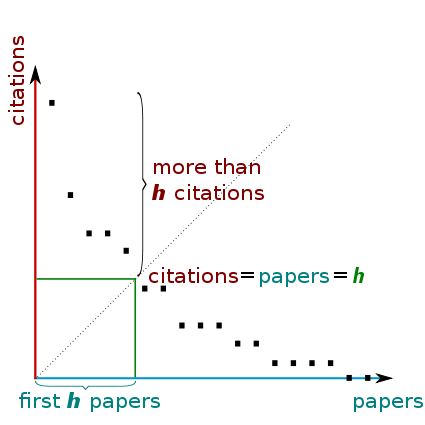
\epsfig{file=figures/hindex.eps}
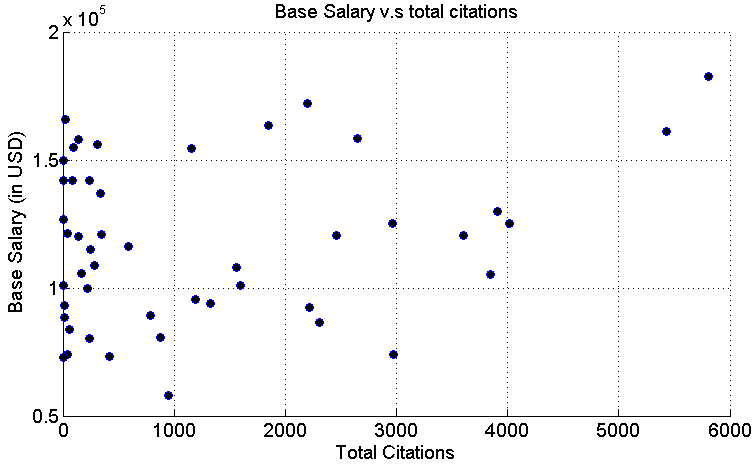
\includegraphics[width=0.5\textwidth]{figures/totalcit.png}
\caption{Plot of base salary versus citations per year.}
\end{figure}

\subsubsection{Citations Per Year}
\label{sectionCitperyear}
Citation counts are accumulated over years. Suppose Prof.~A's paper published 20 years ago got instant attention leading to a huge number of citations, but later on did not really get much attention. The paper would indeed be of value, but if the professor is not writing more papers of good quality or not getting sustained attention from the rest of research community, then total citation count fails to capture this effect of time. In order to overcome this, we can consider citations per year as a measure of centrality~\figref{figCitperyear}. Table~\ref{tableCitperyear} gives the output of running a linear regression on citation per year as a measure of productivity. Since the p-value is less than $2\%$, we can reject the null hypothesis.

\begin{table}[h]
\centering
\label{tableCitperyear}
\caption{Results of Linear Regression with citations per year.}
\begin{tabular} {|l|c|c|}\hline
  $R^2 = 0.601$ & \text{Estimate} &  \text{P-Value} \\ \hline
  \text{Constant} & $56349.2$ & $1.21\times10^{-8}$\\ \hline
 \text{Years Since Ph.~D.} & $2447.57$ & $7.12\times10^{-10}$ \\ \hline
 \text{Citations Per Year} & $45.8953$ & $1.65\times10^{-2}$\\ \hline
 \end{tabular}
\end{table}

\begin{figure}[h]
\label{figCitperyear}
\centering
%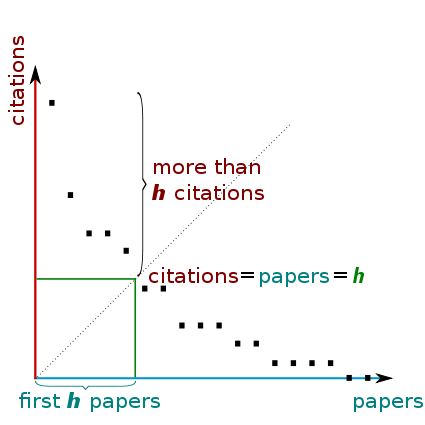
\epsfig{file=figures/hindex.eps}
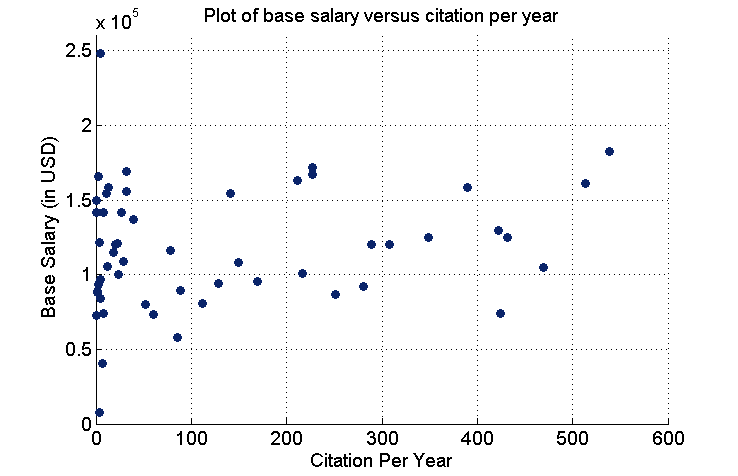
\includegraphics[width=0.5\textwidth]{figures/citperyr.png}
\caption{Plot of base salary versus citations per year.}
\end{figure}



\subsubsection{PageRank}
\label{sectionPageRank}
PageRank~\cite{page1999} is a Eigenvector based centrality measure. It tries to capture the relative importance of a node based on the rank of it neighbors.

\begin{equation}
  \label{eqnPageRank}
  PageRank(A) = \frac{1-\alpha}{N} + \alpha \sum_{i\in\mathcal{N}_A}\frac{PageRank(i)}{d_{out}(i)}
\end{equation}
where, $\alpha$ is damping factor, $N$ is the total number of nodes, $\mathcal{N}_A = \{i : i\ \text{is a neighbor of A} \}$, $d_{out}$ is the out-degree of node $i$. From the equation~\ref{eqnPageRank} we see that PageRank weighs each in-coming edge by the fraction of the rank of the source node.

In our study, we use $\alpha = 0.85$ which is the typical value of damping factor used in most PageRank computations. Also we set our error tolerance limit to $10^{-5}$ to compute the PageRank numerically using iGraph~\cite{iGraph2006}. We added the PageRank of individual papers to obtain productivity of professor and regressed it against base salary. Table~\ref{tablePageRank} gives the output of this regression, and we see that the p-value is too high to reject null hypothesis.


\begin{table}[h]
\centering
\label{tablePageRank}
\caption{Results of Linear Regression with PageRank.}
\begin{tabular} {|l|c|c|}\hline
  $R^2 = 0.562$ & \text{Estimate} &  \text{P-Value} \\ \hline
  \text{Constant} & $61447.5$ & $1.39\times10^{-9}$\\ \hline
 \text{Years Since Ph.~D.} & $2420.96$ & $3.03\times10^{-9}$ \\ \hline
 \text{PageRank} & $1.1362\times10^{6}$ & $0.1945$\\ \hline
 \end{tabular}
\end{table}



\subsubsection{Change in Citation Count}
\label{sectionDeltacit}

Results in section~\ref{sectionCitcount} and~\ref{sectionCitperyear} suggest correlation between citations and base salary. Salary of a professor is not stagnant. There will be revisions every few years. It would be interesting to see how change in citation count is correlated to change in base salary. From the UC system, we see that there is a change in base salary every two years, in even year. So, we computed biyearly change from $2004$ to $2010$ in salary and citation count and ran a linear regression. Since we are concerned with change in the quantities, we follow the following model,
\begin{equation}
  salary = \beta_1 \Delta\text{Citation}.
\end{equation}

From table~\ref{tableDeltacit}, we see that the p-vale is very low and hence we can reject the null hypothesis.  

\begin{table}[h]
\centering
\label{tableDeltacit}
\caption{Results of Linear Regression with biyearly change in citation and salary.}
\begin{tabular} {|l|c|c|}\hline
  $R^2 = 0.27 $& \text{Estimate} &  \text{P-Value} \\ \hline
 \text{$\Delta Citation$} & $33.4899$ & $6.14\times10^{-12}$ \\ \hline
 \end{tabular}
\end{table}

\begin{figure}[h]
\label{figDeltacit}
\centering
%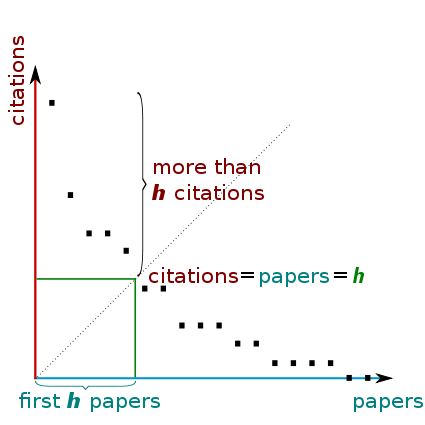
\epsfig{file=figures/hindex.eps}
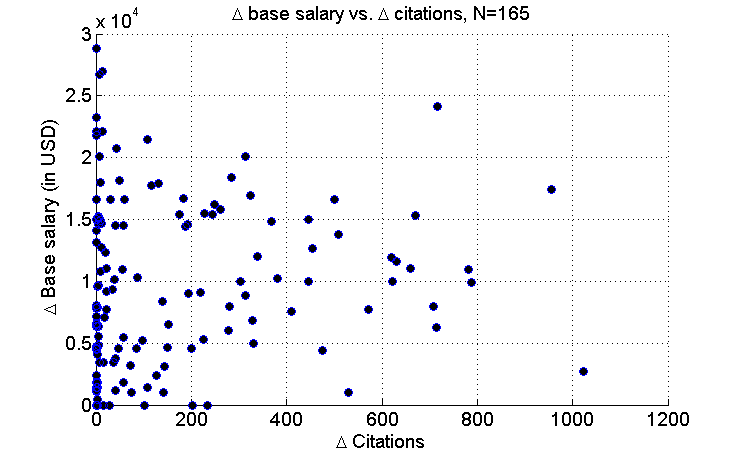
\includegraphics[width=0.5\textwidth]{figures/deltacitations.png}
\caption{Plot of biyearly change in base salary versus change in citations.}
\end{figure}

\subsubsection{h-index}

h-index was introduced by Hirsh~\cite{hirsh2005Hindex} to measure the impact of works by a researcher. It defined as, 
\begin{definition}
  \label{defHindex}
A scientist has index h if h of his/her $N_p$ papers have at least h citations each, and the other $(N_p -h)$ papers have no more than h citations each.  
\end{definition}
 
\begin{figure}[h]
\label{figHindex}
\centering
%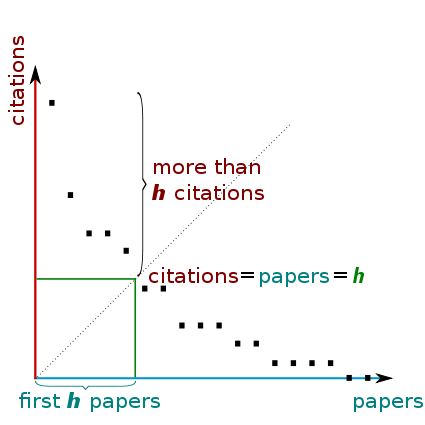
\epsfig{file=figures/hindex.eps}
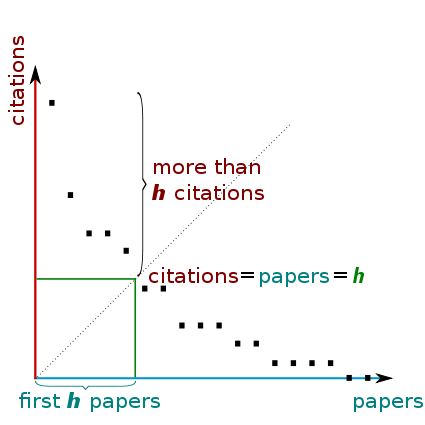
\includegraphics[width=0.4\textwidth]{figures/hindex.png}
\caption{Computing h-index (\small{Courtesy: Wikipedia})}.
\end{figure}

Using this definition~\ref{defHindex} We computed the h-index for professors in our database based on the total citation count of each of their papers. Using this as a measure of productivity we ran a linear regression against base salary (using years since Ph.~D. as secondary variable). Table~\ref{tableHindex} shows the results of this regression. We see that the p-value is too high to reject null hypothesis.

\begin{table}[h]
\centering
\label{tableHindex}
\caption{Results of Linear Regression with h-index.}
\begin{tabular} {|l|c|c|}\hline
  $R^2 = 0.550$ & \text{Estimate} &  \text{P-Value} \\ \hline
  \text{Constant} & $54787.5$ & $6.07\times10^{-7}$\\ \hline
 \text{Years Since Ph.~D.} & $2593.7$ & $1.7\times10^{-9}$ \\ \hline
 \text{h-index} & $262.509$ & $0.39$\\ \hline
 \end{tabular}
\end{table}


\subsubsection{g-index}

In 2006, Leo Egghe~\cite{egghe2006Gindex} suggested a new index to quantify research productivity. It is difined as
\begin{definition}
  \label{defGindex}
  Given a set of articles ranked in decreasing order of the number of citations that they have received, the g-index is the unique largest number such that the top g articles together have received at least $g^2$ citations.
\end{definition}

That is,
\begin{equation}
  \label{eqnGindex}
  g^2 \leq \sum_{i\leq g} c_i
\end{equation}
where, $c_i$ is the number of citations received by paper $i$. Equation~\ref{eqnGindex} can also be re-written as 
\begin{equation}
  g \leq \frac{1}{g} \sum_{i\leq g} c_i
\end{equation}

and hence can be interpreted as $g$ papers of the author have, on average, $g$ citations each.

Based on this definition~\ref{defGindex} of g-index, we computed g-index for each professor in our database, and regressed it against the base salary. The results are in the table~\ref{tableGindex}, from which we see that the p-value is too high and hence we cannot reject null hypothesis.

\begin{figure}[h]
\label{figGindex}
\centering
%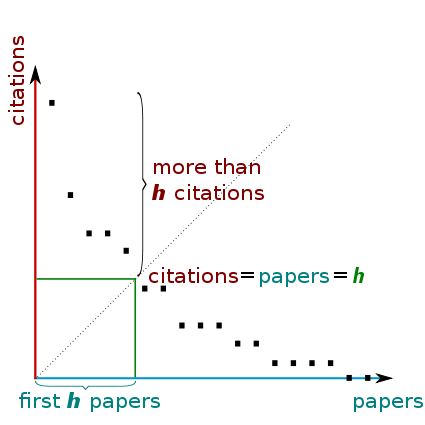
\epsfig{file=figures/hindex.eps}
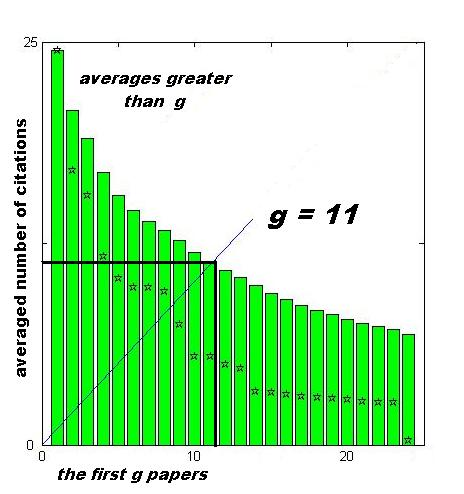
\includegraphics[width=0.4\textwidth]{figures/Gindex1.png}
\caption{Computing g-index (\small{Courtesy: Wikipedia})}.
\end{figure}

\begin{table}[h]
\centering
\label{tableGindex}
\caption{Results of Linear Regression with g-index.}
\begin{tabular} {|l|c|c|}\hline
  $R^2 = 0.547$ & \text{Estimate} &  \text{P-Value} \\ \hline
  \text{Constant} & $55951.3$ & $1.32\times10^{-7}$\\ \hline
 \text{Years Since Ph.~D.} & $2602.33$ & $5.83\times10^{-10}$ \\ \hline
 \text{g-index} & $90.8829$ & $0.55$\\ \hline
 \end{tabular}
\end{table}



%\begin{table*}
%\centering
%\caption{Some Typical Commands}
%\begin{tabular}{|c|c|l|} \hline
%Command&A Number&Comments\\ \hline
%\texttt{{\char'134}alignauthor} & 100& Author alignment\\ \hline
%\texttt{{\char'134}numberofauthors}& 200& Author enumeration\\ \hline
%\texttt{{\char'134}table}& 300 & For tables\\ \hline
%\texttt{{\char'134}table*}& 400& For wider tables\\ \hline\end{tabular}
%\end{table*}
%% end the environment with {table*}, NOTE not {table}!


%\begin{figure}
%\centering
%\epsfig{file=fly.eps}
%\caption{A sample black and white graphic (.eps format).}
%\end{figure}
%
%\begin{figure}
%\centering
%\epsfig{file=fly.eps, height=1in, width=1in}
%\caption{A sample black and white graphic (.eps format)
%that has been resized with the \texttt{epsfig} command.}
%\end{figure}
%

%\begin{figure}
%\centering
%\psfig{file=rosette.ps, height=1in, width=1in,}
%\caption{A sample black and white graphic (.ps format) that has
%been resized with the \texttt{psfig} command.}
%\end{figure}
%

%\begin{figure*}
%\centering
%\epsfig{file=flies.eps}
%\caption{A sample black and white graphic (.eps format)
%that needs to span two columns of text.}
%\end{figure*}
%and don't forget to end the environment with
  %{figure*}, not {figure}!

